\documentclass[10pt]{beamer}
\usetheme[
%%% options passed to the outer theme
%    hidetitle,           % hide the (short) title in the sidebar
%    hideauthor,          % hide the (short) author in the sidebar
%    hideinstitute,       % hide the (short) institute in the bottom of the sidebar
%    shownavsym,          % show the navigation symbols
%    width=2cm,           % width of the sidebar (default is 2 cm)
%    hideothersubsections,% hide all subsections but the subsections in the current section
%    hideallsubsections,  % hide all subsections
    left               % right of left position of sidebar (default is right)
%%% options passed to the color theme
%    lightheaderbg,       % use a light header background
  ]{AAUsidebar}

% If you want to change the colors of the various elements in the theme, edit and uncomment the following lines
% Change the bar and sidebar colors:
%\setbeamercolor{AAUsidebar}{fg=red!20,bg=red}
%\setbeamercolor{sidebar}{bg=red!20}
% Change the color of the structural elements:
%\setbeamercolor{structure}{fg=red}
% Change the frame title text color:
%\setbeamercolor{frametitle}{fg=blue}
% Change the normal text color background:
%\setbeamercolor{normal text}{bg=gray!10}
% ... and you can of course change a lot more - see the beamer user manual.


\usepackage[utf8]{inputenc}
\usepackage[english]{babel}
\usepackage[T1]{fontenc}
% Or whatever. Note that the encoding and the font should match. If T1
% does not look nice, try deleting the line with the fontenc.
\usepackage{helvet}

% colored hyperlinks
\newcommand{\chref}[2]{%
  \href{#1}{{\usebeamercolor[bg]{AAUsidebar}#2}}%
}

\title[Double Tracking Antennas for UAS Communication]% optional, use only with long paper titles
{Control and Automantion}

\subtitle{v.\ 1.3.0}  % could also be a conference name

\date{\today}

\author[Group CA832] % optional, use only with lots of authors
{
  Jesper Kjær Nielsen\\
  \href{mailto:jkn@es.aau.dk}{{\tt jkn@es.aau.dk}}
}
% - Give the names in the same order as they appear in the paper.
% - Use the \inst{?} command only if the authors have different
%   affiliation. See the beamer manual for an example

\institute[
%  {\includegraphics[scale=0.2]{aau_segl}}\\ %insert a company, department or university logo
  Dept.\ of Electronic Systems\\
  Aalborg University\\
  Denmark
] % optional - is placed in the bottom of the sidebar on every slide
{% is placed on the title page
  Department of Electronic Systems\\
  Aalborg University\\
  Denmark
  
  %there must be an empty line above this line - otherwise some unwanted space is added between the university and the country (I do not know why;( )
}


% specify a logo on the titlepage (you can specify additional logos an include them in 
% institute command below
\pgfdeclareimage[height=1.5cm]{titlepagelogo}{AAUgraphics/aau_logo_new} % placed on the title page
%\pgfdeclareimage[height=1.5cm]{titlepagelogo2}{graphics/aau_logo_new} % placed on the title page
\titlegraphic{% is placed on the bottom of the title page
  \pgfuseimage{titlepagelogo}
%  \hspace{1cm}\pgfuseimage{titlepagelogo2}
}


\begin{document}
% the titlepage
{\aauwavesbg%
\begin{frame}[plain,noframenumbering] % the plain option removes the sidebar and header from the title page
  \titlepage
\end{frame}}
%%%%%%%%%%%%%%%%

% TOC
\begin{frame}{Agenda}{}
\tableofcontents
\end{frame}
%%%%%%%%%%%%%%%%

\section{Introduction}

\begin{frame}{Introduction}{}
\begin{figure}[H]
\centerline{
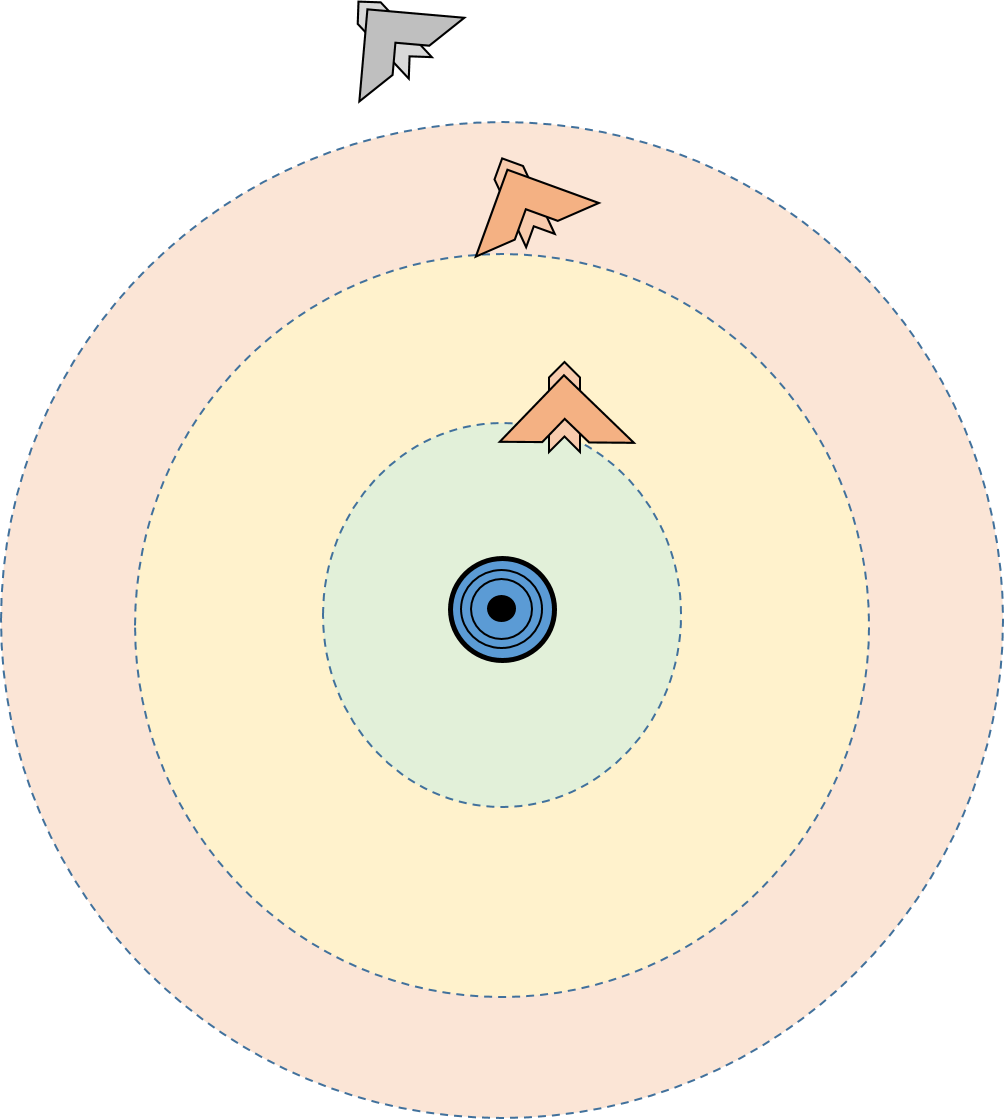
\includegraphics[scale=0.35]{figures/intro.png}}
\label{fig:overview}
\end{figure}
\end{frame}



\subsection{Hardware}

\begin{frame}{Hardware}{}
  \begin{block}{Unmanned Aicraft System (UAS)}
    \begin{enumerate}
      \item Unmanned Aircraft (UA)
      \item Ground Station (GS)
      \item Antennas
      \item DC Servomotor
    \end{enumerate}
  \end{block}
\end{frame}


\chapter{Frames}\label{ch:frames}

In navigation, guidance, and control of an aircraft or rotorcraft, there are several
coordinate systems (or frames) intensively used in design and analysis. For ease of references, in this chapter the coordinate systems adopted in this project have been sumarized, which include:

\begin{itemize}
\item{The Geodetic Coordinate System}
\item{The Earth-Centered Earth-Fixed (ECEF) Coordinate System}
\item{The local North-East-Down (NED) Coordinate System}
\item{The vehicle-carried NED Coordinate System}
\item{The Body Coordinate System}
\end{itemize}

The relationships among these coordinate systems, i.e., the coordinate transformations, are also introduced. We need to point out that small UAs are normally used at low speeds in relatively small regions (non trans-oceanic travels), due to their inherent mechanical design and power limitation. This is crucial to some simplifications made in the coordinate transformation, e.g., omitting unimportant items in the transformation between the local NED frame and the body frame. For the same reason, partial transformation relationships provided in this chapter are not suitable for describing flight situations in which the rotation of the Earth is taken into account.
\subsection{Telecommunication}

\begin{frame}{Telecommunication}{}

  \begin{block}{Line-Of-Sight (LOS) Propagation}

  \end{block}
  
  \begin{block}{Link Budget}

  \end{block}

  \begin{block}{Fresnel Zones}

  \end{block}

  \begin{block}{MAVLink Protocol}

  \end{block}

\end{frame}

\chapter{Modelling}\label{ch:model}

!!! INTRO !!!

??? State-space model ???



% list of the themes and options
% {\setbeamercolor{frametitle}{use=structure,fg=structure.fg,bg=white}
% \begin{frame}{User Interface}{Loading the Theme and Theme Options}
%   \begin{block}{The Color Theme}
%     You can load the color theme directly by\\
%     {\tt \textbackslash usecolortheme[<options>]\{AAUsidebar\}}\\
%     Currently, the only theme option is
%     \begin{itemize}
%       \item {\tt lightheaderbg}: use a light header background (currently, it is white). 
%     \end{itemize}
%     This option creates the light header used on this slide.
%   \end{block}
%   \pause
%   \begin{block}{The Color Element {\tt AAUsidebar}}
%     The color theme defines a new beamer color element named {\tt AAUsidebar} whose foreground and background colors are
%     \begin{itemize}
%       \item fg: {\usebeamercolor[fg]{AAUsidebar}light blue (\{RGB\}\{194,193,204\})}
%       \item bg: {\usebeamercolor[bg]{AAUsidebar}dark blue (\{RGB\}\{33,26,82\})}
%     \end{itemize}
%     You can use these colors in the standard beamer way by using the command
%     {\tt \textbackslash usebeamercolor[<fg or bg>]\{AAUsidebar\}}. See the beamer manual for instructions.
%   \end{block}
% \end{frame}
% }
%%%%%%%%%%%%%%%%

{\aauwavesbg
\begin{frame}[plain,noframenumbering]
  \finalpage{Thank you for flying with us!}
\end{frame}}
%%%%%%%%%%%%%%%%

\end{document}
